\section{はじめに}
所与の領域を1人または複数の巡査が動き回り,
その領域内の指定された場所を十分な頻度で訪れることを
警邏(patrolling)という\cite{chen2013fence, coene2011charlemagne, czyzowicz2011boundary}.


本稿では,与えられた距離空間$U$内を速さ$1$以下の巡査$m$人が動きまわることにより,
集合$V \subseteq U$に属する多くの点に十分な頻度で訪れるという目標を考える.
すなわち次のような問題である.

巡査$i \in \{1, \ldots, m\}$の$U$上の運行$a _i \colon \Rset \to U$とは,
各時刻$t \in \Rset$における位置$a _i (t) \in U$を定めるものであって,
任意の時刻$s$,$t \in \Rset$に対し$a _i (s)$と$a _i (t)$の距離が$\abs{s - t}$を超えないものをいう.
巡査$m$人による$U$上の運行とは,
全巡査の運行を定めた組
$A = (a _1, \dots, a _m)$をいう.
運行$A = (a _1, \dots, a _m)$
が点$v \in U$を{\idletime}$q \geq 0$で警備するとは,
長さ$q$のどの時間区間にも
いずれかの巡査が$v$を少くとも一度は訪れる
(任意の時刻$t \in \Rset$に対して
巡査$i$と時刻$\tau \in [t, t + q)$が存在し
$a _i (\tau) = v$)ことをいう.
\red{(←$q = 0$のときおかしい?)}

$U$の有限な部分集合$V$があり,$V$の各点には利得および{\idletime}と呼ばれる非負整数が定まっている.
運行$A$が点集合$W \subseteq V$を警邏するとは,
各点$v \in W$に対し$A$が$v$を警備することをいう.
そのような運行が存在するとき$W$は$m$人により警邏可能であるという.

\begin{cooperativepatrollingproblem}
  巡査の人数$m$と距離空間$U$内の点集合$V$および
  $V$の各点の利得と{\idletime}が与えられたとき,
  $m$人の巡査により警邏可能な頂点集合のうち利得の和が最大となるものを求めよ.
\end{cooperativepatrollingproblem}

距離空間$U$といっても,$V$の点同士の測地距離のみが重要である.
そこでこの問題の入力は,
$V$を頂点集合とし辺に非負整数の長さがついた無向グラフと考えることにする.

この問題は,巡査が一人かつ
全点の利得と{\idletime}が等しい場合に限っても,
ハミルトン路問題からの帰着により
NP困難である\cite[Theorem~8]{coene2011charlemagne}.
そこでグラフの形状を限ったときにどのようになるかを調べる.

一つの頂点が複数の巡査の訪問により警備され得ることに注意されたい.
例えば図\ref{figure: cooperative}左はそのような運行の例である.
\begin{figure}
  \begin{center}
    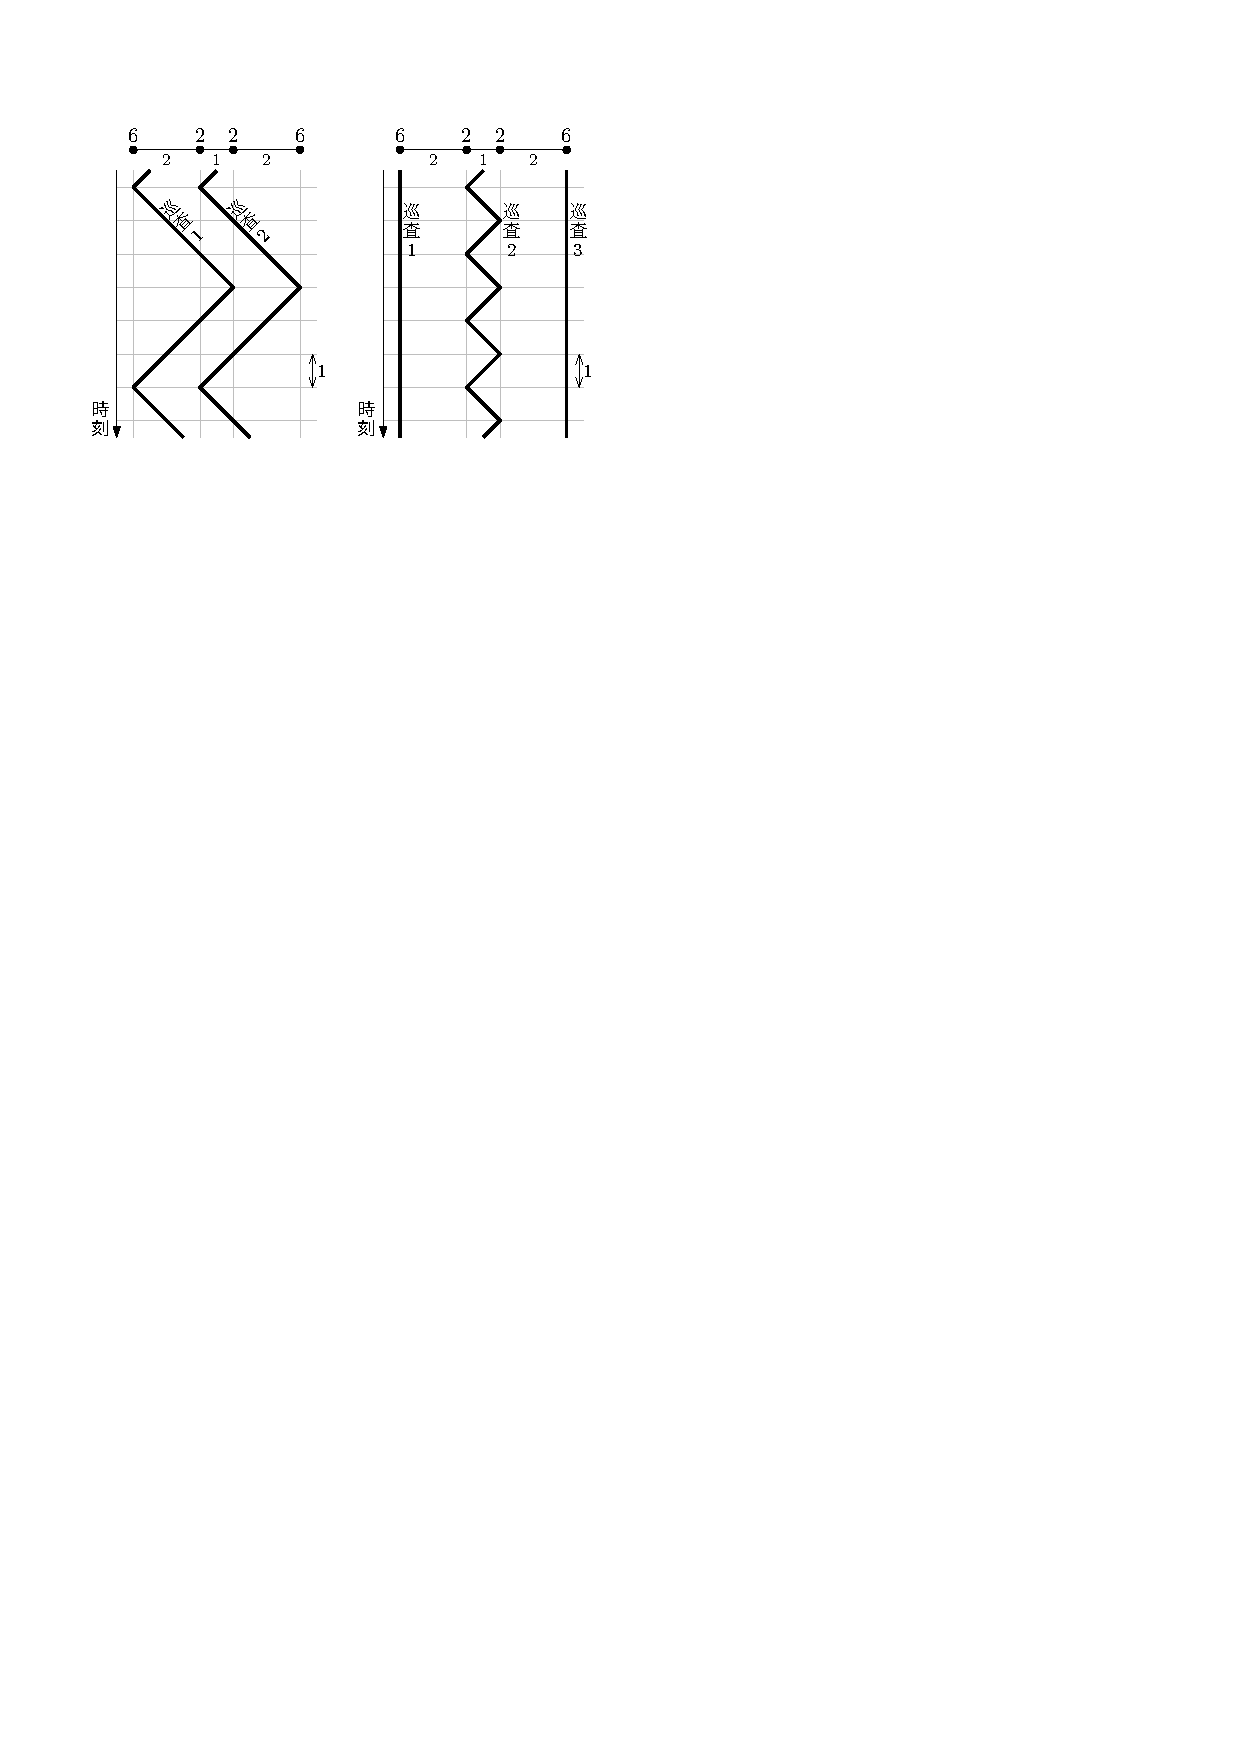
\includegraphics[scale=1.0]{\figdir/cooperative.pdf}
    \caption{図の上部に描かれている四点からなるグラフの全点を警邏する二つの運行.
      頂点と辺に書かれた数は,それぞれ{\idletime}と距離である.
      左図の運行では二人の巡査が協力して中央の二点を間隔$2$で警備している.
      これを禁じ,各点がいずれかの巡査により単独警備されることを求める場合は,
      右図のように三人の巡査を要する.}
    \label{figure: cooperative}
  \end{center}
\end{figure}
Coeneら\cite{coene2011charlemagne}は似た問題を扱っているが,
このような協力を許さず,
図\ref{figure: cooperative}右のように
各頂点を専ら一人の巡査が「担当」することを要求している.
つまり,各頂点$v \in W$が単独警備される(すなわち
或る一人の巡査がおり,
その巡査のみの運行が$\{v\}$を警邏する)ことを要求しているのである.
対比のため本稿ではこの問題を{\assignedPatProb}と呼ぶことにする
(\cite{coene2011charlemagne}ではMPLPPと称している).
Coeneら\cite{coene2011charlemagne}の諸結果においては,
この単独警備という限定が,
多項式時間算法の設計にも困難性の証明にも重要な役割を果している.
この限定を外したときの様子を調べるのが本稿の目的である.

本稿ではグラフの形状として
線分,星と,すべての枝の長さが等しい完全グラフの3種類を扱うこととし
(図\ref{figure: graph_classes}),
以降はそれぞれを {\graphLine}, {\graphStar}, {\graphUnit}と呼ぶ.
\begin{figure}
  \begin{center}
    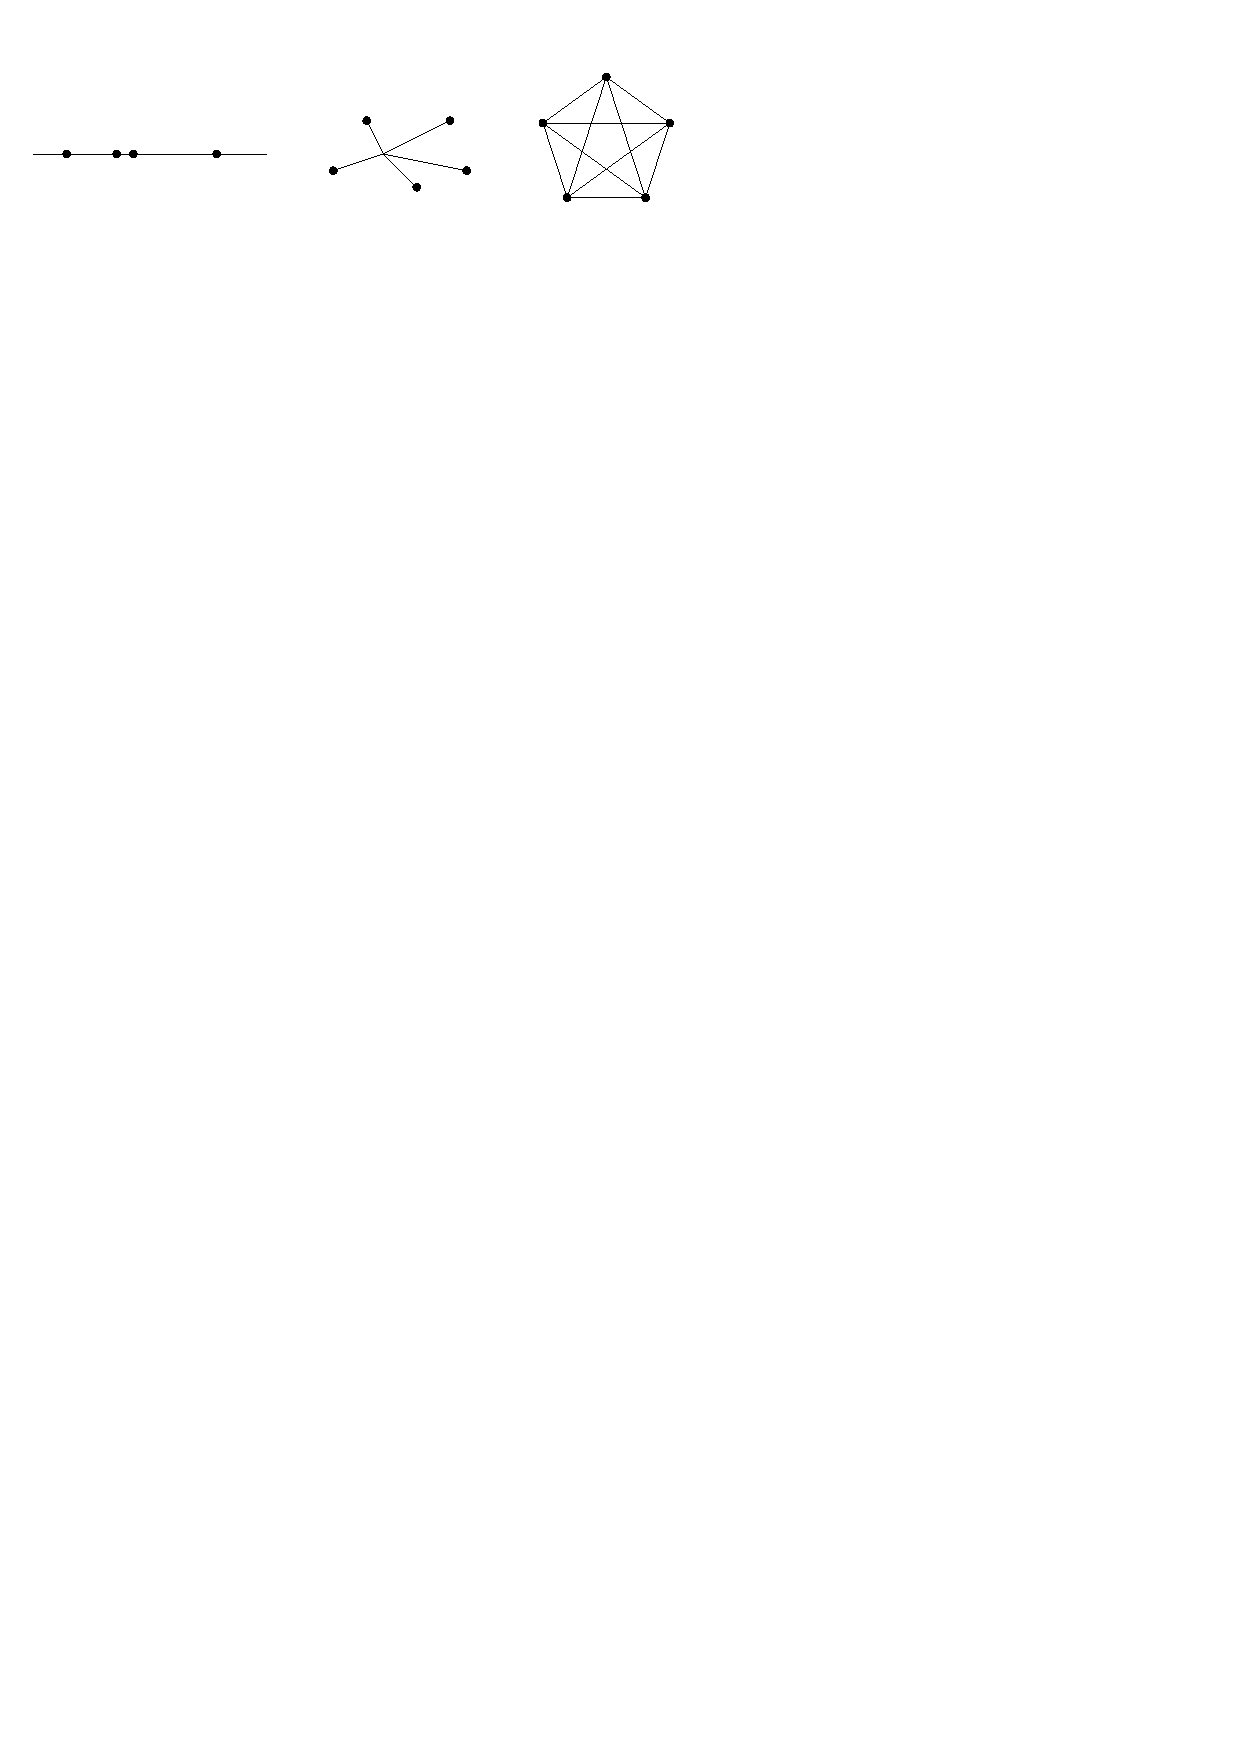
\includegraphics[scale=1.0]{\figdir/graph_classes.pdf}
    \caption{本論文では{\graphLine}(左),{\graphStar}(中),{\graphUnit}(右,但し各辺の長さが等しい)を扱う.{\graphStar}は葉のみを警備の対象とする(中央の点は移動の途中で使うのみであり,{\idletime}は定められていない).}
    \label{figure: graph_classes}
  \end{center}
\end{figure}
{\graphStar}では葉のみに{\idletime}が定められている(中心は警備の対象としない).
{\patProb}においては前述のとおり頂点同士の測地距離のみが重要であるため,
{\graphUnit}は,その各辺の長さを$d$とすると,
同じ頂点数で辺の長さがすべて$d/2$である{\graphStar}と同一視できることから,
{\graphUnit}は{\graphStar}の特殊な場合である.


% 巡査協力なしの結果との比較
{\patProb}についての我々の結果と,
{\assignedPatProb}についてのCoeneらの結果を,
グラフの形ごとに比較すると次のようになる.
それぞれ\ref{section: line},\ref{section: star},\ref{section: unit}節で述べる.
\begin{itemize}
  \item 
    グラフが{\graphLine}の場合は,
    {\assignedPatProb}は動的計画法により多項式時間で解けることが
    示されていた\cite[Theorem~11]{coene2011charlemagne}が,
    その正しさは非協力の設定に強く依存している.
    本稿では{\patProb}について,
    全点の{\idletime}が等しい場合には多項式時間で解ける
    (定理\ref{theo:LineEqualTimelimit}).
  \item
    グラフが{\graphStar}の場合は,
    全点の利得と{\idletime}が等しい場合に限っても,
    {\assignedPatProb}はNP困難であることが示されていた\cite[Theorem~10]{coene2011charlemagne}.
    本稿では,この場合の{\patProb}は多項式時間で解けるという興味深い結果を得る(定理**).
    なお利得または{\idletime}を一般にすると,
    巡査が一人であっても(したがって担当の有無に関わらず)
    NP困難であることがわかっている\cite[Theorems 5 and 6]{coene2011charlemagne}.
  \item 
    グラフが{\graphUnit}の場合は,
    全点の{\idletime}が等しい場合は{\patProb}が多項式時間で解けることを示す(定理**).
    グラフが{\graphStar}の場合は全点の{\idletime}が等しくても利得が一般だとNP困難になるので,
    これにより{\graphUnit}は{\graphStar}よりも簡単に解ける場合となっていることが分かる.
\end{itemize}


{\graphLine}と{\graphUnit}については
{\idletime}が一般の場合については多項式時間アルゴリズムやNP困難性を示すのが難しく未解決である.
これらの未解決な状況については,
{\idletime}の代わりに以下に定義する{\exactidletime}を警備の条件とする問題も考えた.

\begin{defi}
  運行$A = (a _1, \ldots, a _m)$が
  点$v \in U$を{\exactidletime}$(q, r)$で警備するとは,
  任意の時刻$t := q k + r (k \in \Zset)$に対し
  巡査$i$が存在し
  $a _i (t) = v$
  であることをいう.
\end{defi}

{\exactidletime}による{\patProb}は以下のように定義される.

\begin{timeSpecifiedCooperativePatrollingProblem}
  巡査の人数$m$と距離空間$U$内の点集合$V$および
  $V$の各点の利得と{\exactidletime}が与えられたとき,
  $m$人の巡査により警邏可能な頂点集合のうち利得の和が最大となるものを求めよ.
\end{timeSpecifiedCooperativePatrollingProblem}

判定問題は以下のようになる.

\begin{timeSpecifiedCooperativePatrollingProblemDecision}
  巡査の人数$m$と距離空間$U$内の点集合$V$および
  $V$の各点の{\exactidletime}が与えられたとき,
  $m$人の巡査により$V$を警邏可能か判定せよ.
\end{timeSpecifiedCooperativePatrollingProblemDecision}


{\graphLine}については{\timeSpecifiedPatProbDecision}を解く貪欲アルゴリズムを示す(定理\ref{}).
{\graphUnit}については{\timeSpecifiedPatProbDecision}がNP困難であることを示す(定理\ref{}).




\subsection*{関連研究}

\red{(あまり本筋に関係ない関連研究は、論文冒頭ではなくこの辺に書くのも手)}

% 警邏に関する研究には様々な問題設定があり,
% 例えば線分や閉路のような交わりの無い1次元的な領域のすべての点を警邏する
% 塀の警邏(Fence Patrolling)問題~\cite{chen2013fence, czyzowicz2011boundary}や,
% より一般的なグラフで辺全体ではなく頂点を警備する警邏問題~\cite{coene2011charlemagne},
% グラフと巡査が与えられて警邏可能かを判定する問題だけでなく,
% 塀の警邏問題においてなるべく長い塀を警邏する問題~\cite{czyzowicz2011boundary}や
% 全体の訪問の待ち時間の最大値を最小化する問題~\cite{chen2013fence}
% なども考えられている.
% \red{(加筆予定)}

また,{\graphLine}や{\graphStar}は木の特別な場合である.
